\documentclass[journal,12pt,twocolumn]{IEEEtran}

\usepackage{setspace}
\usepackage{gensymb}
\singlespacing
\usepackage[cmex10]{amsmath}

\usepackage{amsthm}

\usepackage{mathrsfs}
\usepackage{txfonts}
\usepackage{stfloats}
\usepackage{bm}
\usepackage{cite}
\usepackage{cases}
\usepackage{subfig}

\usepackage{longtable}
\usepackage{multirow}

\usepackage{enumitem}
\usepackage{mathtools}
\usepackage{steinmetz}
\usepackage{tikz}
\usepackage{circuitikz}
\usepackage{verbatim}
\usepackage{tfrupee}
\usepackage[breaklinks=true]{hyperref}
\usepackage{graphicx}
\usepackage{tkz-euclide}

\usetikzlibrary{calc,math}
\usepackage{listings}
    \usepackage{color}                                            %%
    \usepackage{array}                                            %%
    \usepackage{longtable}                                        %%
    \usepackage{calc}                                             %%
    \usepackage{multirow}                                         %%
    \usepackage{hhline}                                           %%
    \usepackage{ifthen}                                           %%
    \usepackage{lscape}     
\usepackage{multicol}
\usepackage{chngcntr}

\DeclareMathOperator*{\Res}{Res}

\renewcommand\thesection{\arabic{section}}
\renewcommand\thesubsection{\thesection.\arabic{subsection}}
\renewcommand\thesubsubsection{\thesubsection.\arabic{subsubsection}}

\renewcommand\thesectiondis{\arabic{section}}
\renewcommand\thesubsectiondis{\thesectiondis.\arabic{subsection}}
\renewcommand\thesubsubsectiondis{\thesubsectiondis.\arabic{subsubsection}}


\hyphenation{op-tical net-works semi-conduc-tor}
\def\inputGnumericTable{}                                 %%

\lstset{
%language=C,
frame=single, 
breaklines=true,
columns=fullflexible
}
\begin{document}

\newcommand{\BEQA}{\begin{eqnarray}}
\newcommand{\EEQA}{\end{eqnarray}}
\newcommand{\define}{\stackrel{\triangle}{=}}
\bibliographystyle{IEEEtran}
\raggedbottom
\setlength{\parindent}{0pt}
\providecommand{\mbf}{\mathbf}
\providecommand{\pr}[1]{\ensuremath{\Pr\left(#1\right)}}
\providecommand{\qfunc}[1]{\ensuremath{Q\left(#1\right)}}
\providecommand{\sbrak}[1]{\ensuremath{{}\left[#1\right]}}
\providecommand{\lsbrak}[1]{\ensuremath{{}\left[#1\right.}}
\providecommand{\rsbrak}[1]{\ensuremath{{}\left.#1\right]}}
\providecommand{\brak}[1]{\ensuremath{\left(#1\right)}}
\providecommand{\lbrak}[1]{\ensuremath{\left(#1\right.}}
\providecommand{\rbrak}[1]{\ensuremath{\left.#1\right)}}
\providecommand{\cbrak}[1]{\ensuremath{\left\{#1\right\}}}
\providecommand{\lcbrak}[1]{\ensuremath{\left\{#1\right.}}
\providecommand{\rcbrak}[1]{\ensuremath{\left.#1\right\}}}
\theoremstyle{remark}
\newtheorem{rem}{Remark}
\newcommand{\sgn}{\mathop{\mathrm{sgn}}}
\providecommand{\abs}[1]{\vert#1\vert}
\providecommand{\res}[1]{\Res\displaylimits_{#1}} 
\providecommand{\norm}[1]{\lVert#1\rVert}
%\providecommand{\norm}[1]{\lVert#1\rVert}
\providecommand{\mtx}[1]{\mathbf{#1}}
\providecommand{\mean}[1]{E[ #1 ]}
\providecommand{\fourier}{\overset{\mathcal{F}}{ \rightleftharpoons}}
%\providecommand{\hilbert}{\overset{\mathcal{H}}{ \rightleftharpoons}}
\providecommand{\system}{\overset{\mathcal{H}}{ \longleftrightarrow}}
	%\newcommand{\solution}[2]{\textbf{Solution:}{#1}}
\newcommand{\solution}{\noindent \textbf{Solution: }}
\newcommand{\cosec}{\,\text{cosec}\,}
\providecommand{\dec}[2]{\ensuremath{\overset{#1}{\underset{#2}{\gtrless}}}}
\newcommand{\myvec}[1]{\ensuremath{\begin{pmatrix}#1\end{pmatrix}}}
\newcommand{\mydet}[1]{\ensuremath{\begin{vmatrix}#1\end{vmatrix}}}
\numberwithin{equation}{subsection}
\makeatletter
\@addtoreset{figure}{problem}
\makeatother
\let\StandardTheFigure\thefigure
\let\vec\mathbf
\renewcommand{\thefigure}{\theproblem}
\def\putbox#1#2#3{\makebox[0in][l]{\makebox[#1][l]{}\raisebox{\baselineskip}[0in][0in]{\raisebox{#2}[0in][0in]{#3}}}}
     \def\rightbox#1{\makebox[0in][r]{#1}}
     \def\centbox#1{\makebox[0in]{#1}}
     \def\topbox#1{\raisebox{-\baselineskip}[0in][0in]{#1}}
     \def\midbox#1{\raisebox{-0.5\baselineskip}[0in][0in]{#1}}
\vspace{3cm}
\title{Assignment 1}
\author{Vijay Varma - AI20BTECH11012}
\maketitle
\newpage
\bigskip
\renewcommand{\thefigure}{\theenumi}
\renewcommand{\thetable}{\theenumi}
%
Download latex-tikz codes from 
%
\begin{lstlisting}
https://github.com/KBVijayVarma/EE3900/tree/main/Assignment_1
\end{lstlisting}
%
Download python code from 
%
\begin{lstlisting}
https://github.com/KBVijayVarma/EE3900/tree/main/Assignment_1
\end{lstlisting}
\section*{\textbf{Problem (Ramsey-1.1 Points-Q.8)}}
Prove that the points \myvec{-1\\0}, \myvec{0\\3}, \myvec{3\\2} and \myvec{2\\-1} are the vertices of a square.
\section*{Solution}
Let the given points be
\begin{equation}
\vec{A} = \myvec{-1\\0}, \vec{B} = \myvec{0\\3}, \vec{C} = \myvec{3\\2}, \vec{D} = \myvec{2\\-1}
\end{equation}
We know that the distance between the points $\vec{P}$($x_1$,$y_1$) and $\vec{Q}$($x_2$,$y_2$) is given by
\begin{equation}
||\vec{Z}|| = ||\vec{P} - \vec{Q}||
\end{equation}

Now computing the distances between the points $\vec{A},\vec{B},\vec{C},\vec{D}$,
\begin{align}
    \overline{\rm AB} &= ||\vec{A} - \vec{B}|| = \sqrt{(-1-0)^2 + (0-3)^2} = \sqrt{10}\\
    \overline{\rm BC} &= ||\vec{B} - \vec{C}|| = \sqrt{(0-3)^2 + (3-2)^2} = \sqrt{10}\\
    \overline{\rm CD} &= ||\vec{C} - \vec{D}|| = \sqrt{(3-2)^2 + (2-(-1))^2} = \sqrt{10}\\
    \overline{\rm DA} &= ||\vec{D} - \vec{A}|| = \sqrt{(2-(-1))^2 + (-1-0)^2} = \sqrt{10}\\
    \overline{\rm AC} &= ||\vec{A} - \vec{C}|| = \sqrt{(-1-3)^2 + (0-2)^2} = \sqrt{20}\\
    \overline{\rm BD} &= ||\vec{B} - \vec{D}|| = \sqrt{(0-2)^2 + (3-(-1))^2} = \sqrt{20}
\end{align}

Here, the Sides of the Quadrilateral $\overline{\rm AB}$, $\overline{\rm BC}$, $\overline{\rm CD}$, $\overline{\rm DA}$ are of equal length $\sqrt{10}$ units.

The Diagonals $\overline{\rm AC}$, $\overline{\rm BD}$ are also of equal length $\sqrt{20}$ units.\\

Now, let us check if the Diagonals $\overline{\rm AC}$ and $\overline{\rm BD}$ are perpendicular by using Orthogonality Condition,
\begin{equation}
    (\vec{A} - \vec{C})^T(\vec{B} - \vec{D}) = 0
\end{equation}
We have,
\begin{align}
 \vec{A} - \vec{C} &= (-1-3, 0-2) \\
 \vec{A} - \vec{C} &= \myvec{-4\\-2} \\
 \vec{B} - \vec{D} &= (0-2, 3-(-1)) \\
 \vec{B} - \vec{D} &= \myvec{-2\\4}
\end{align}

For orthogonality, product of transpose of one and other must be 0. Here, checking for

\begin{align}
    (\vec{A} - \vec{C})^T(\vec{B} - \vec{D}) &= \myvec{-4\\-2}^T\myvec{-2\\4} \\
    &= 0
\end{align}

Hence, using Orthogonality, Diagonal $\overline{\rm AC}$ is perpendicular to Diagonal $\overline{\rm BD}$.

$\therefore \overline{\rm AC} \perp \overline{\rm CD}$

Since, the Quadrilateral ABCD has 4 equal sides, equal diagonals perpendicular to each other, Hence it is a Square.

Therefore, ABCD is a square.

Hence, the 4 points $\vec{A},\vec{B},\vec{C},\vec{D}$ are vertices of a Square. \\\\\\\\\\\\\\\\\\\\\\

\begin{figure}[htp]
    \centering
    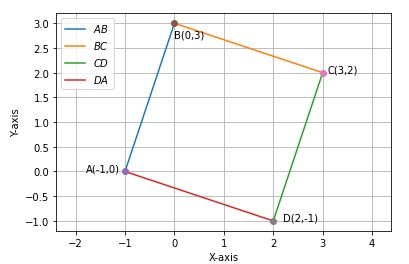
\includegraphics[width=\columnwidth,height=5cm]{fig.jpg}
    \caption{Plot}
    \label{fig:label}
\end{figure}
This can be verified from the Figure \ref{fig:label}.


\end{document}